\clearpage
\chapter{Traversing $\epsilon$ transitions in NFA}

\section{Aim}
To design and implement a C-program that accepts a Non-deterministic Finite Automaton (NFA) and computes $\epsilon$ closure for each states.

\section{Algorithm}

\begin{algorithm}[H]
	\caption{An algorithm to compute $\epsilon$ closure of a state}
	\begin{algorithmic}
		\Procedure{findEpsilionTrans}{$visited, fromState$}
		\State \Comment{visited : Stack of visited states}
		\State \Comment{fromState : Current state to find closure}
		
		\If{$fromstate \in visited$}
		\State return $visited$
		\EndIf
		
		\State $push(visited, fromState)$
		
		\ForAll{$transition \in fromState.transitions$}
		\If{$transition.symbol == \epsilon $}
		\State $visited = $ \Call{findEpsilonTrans}{visited, transition.toState}
		\EndIf
		\EndFor
		\EndProcedure
	\end{algorithmic}
\end{algorithm}

\subsubsection*{Realization of NFA using linked list}

\begin{figure}[H]
	\centering
	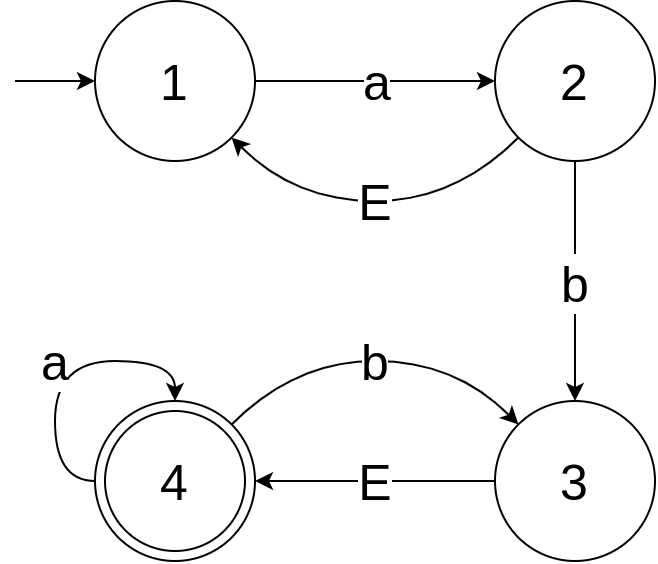
\includegraphics[height=2in]{../EXP4/NFA_realization-NFA.png}
	\caption{NFA}
\end{figure}

\begin{figure}[H]
	\centering
	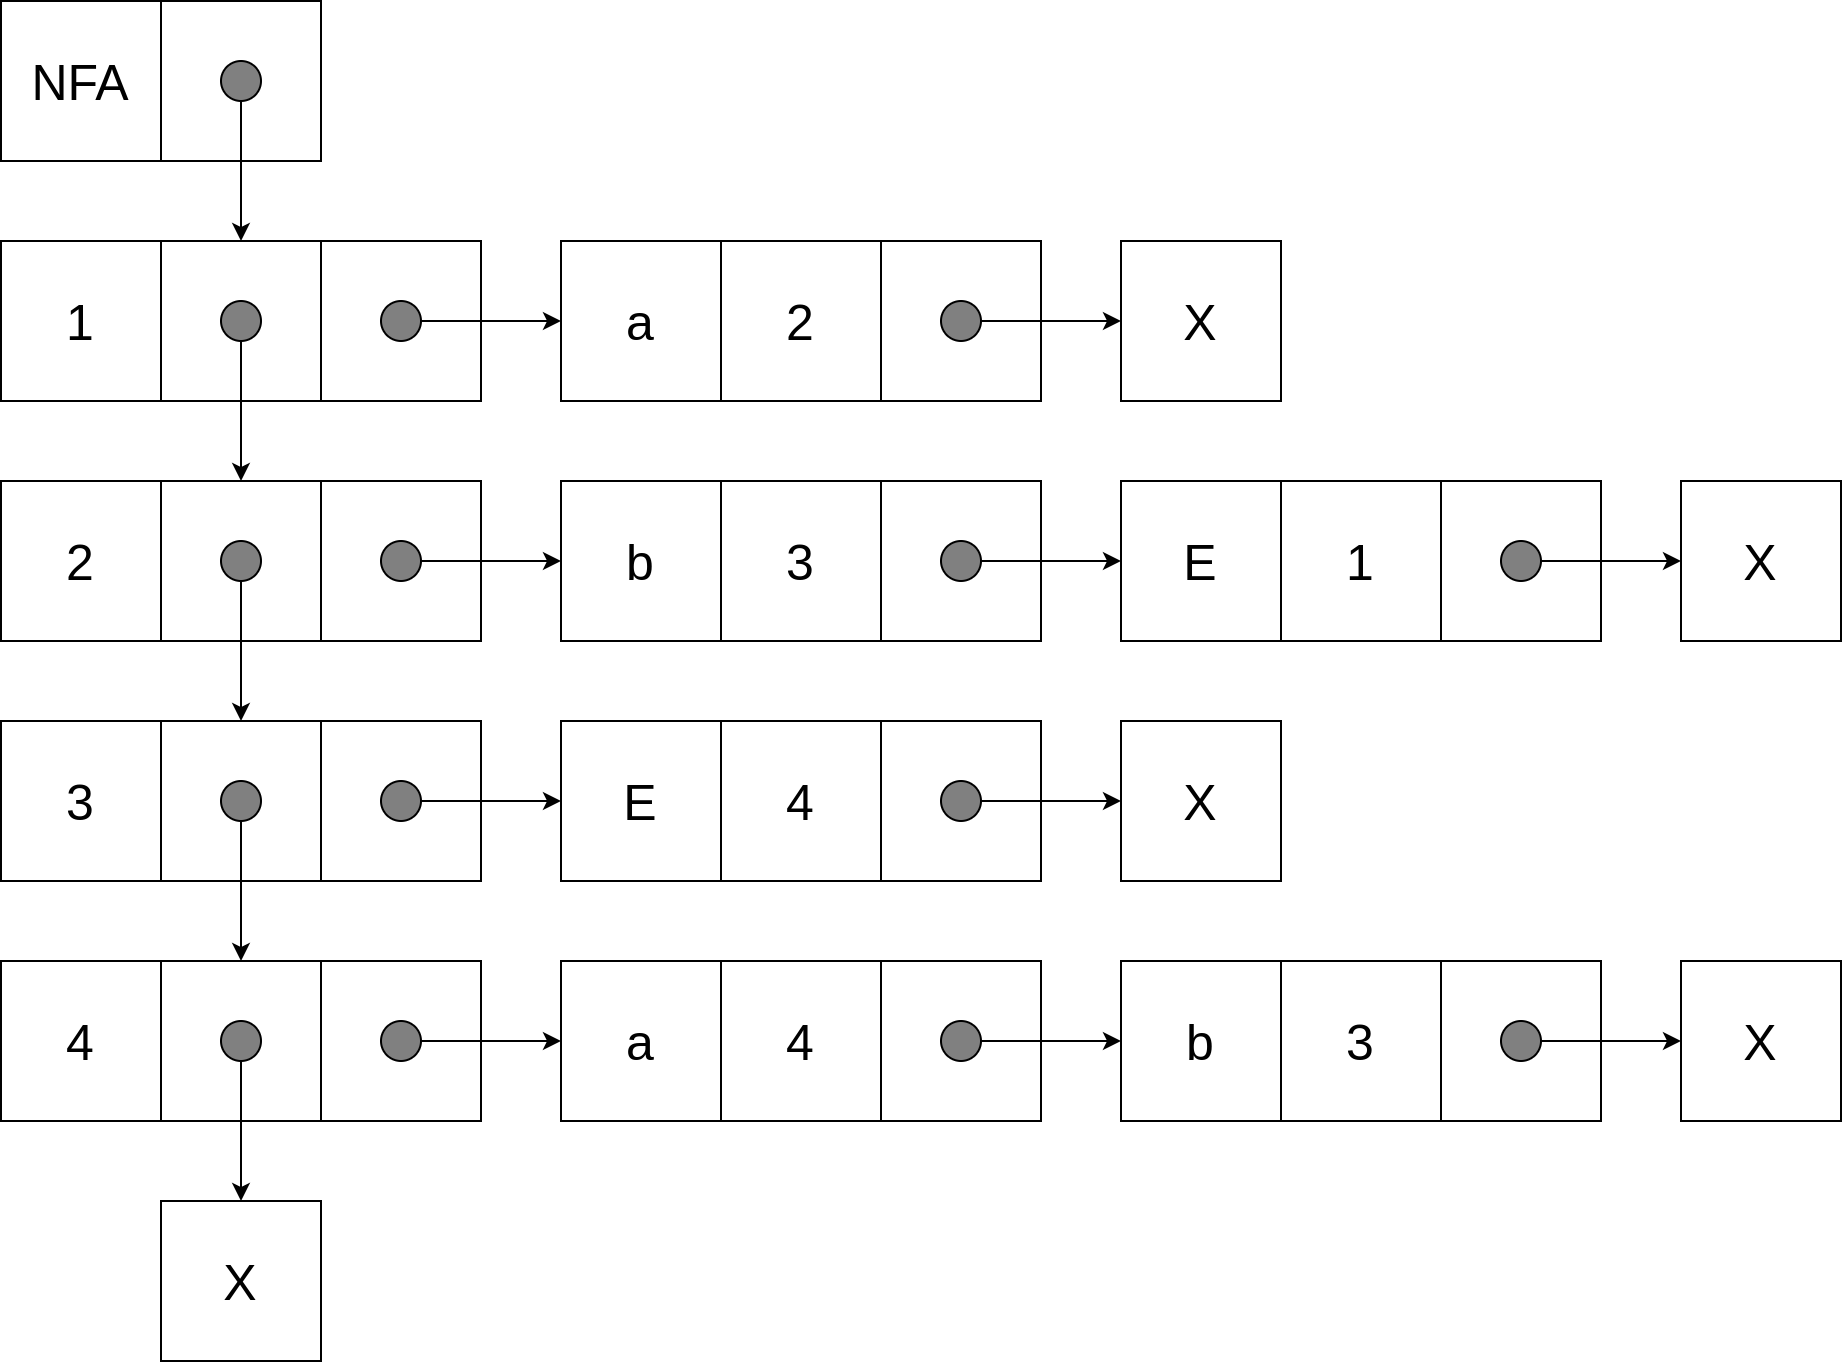
\includegraphics[height=2.5in]{../EXP4/NFA_realization-LinkedList.png}
	\caption{NFA realization via linked list}
\end{figure}
\section{C-Program}
\lstinputlisting[style=CStyle]{../EXP4/epsilonNFA.c}

\section{Output}
\lstinputlisting[style=plain]{../EXP4/output.txt}

\section{Result}
The program compiled successfully and identified $\epsilon$ closure for each states in the given NFA.